\documentclass[tikz,border=5pt]{standalone}
\usepackage{fourier}
\usetikzlibrary{hobby}
\begin{document}
\def\xx{1}
\def\yy{2}
\def\dd{1}
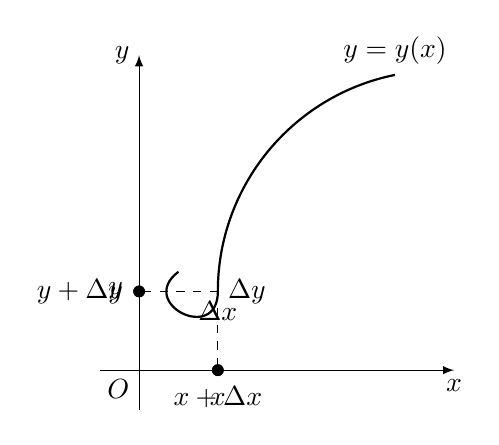
\begin{tikzpicture}[mydot/.style={circle,fill,inner sep=1.5pt}]
  \draw[-latex] (-.5,0) -- (4,0) node[below] {$x$};
  \draw[-latex] (0,-.5) -- (0,4) node[left] {$y$};
  \coordinate (O) at (0,0);
  \coordinate (A) at (\xx,\yy);
  \coordinate (B) at ({\xx+\dd},{\yy+\dd});
  \draw[thick] (A) -- node[below] {$\Delta x$} (A -| B) -- node[right] {$\Delta y$} (B);
  \draw[dashed] 
    (A) -- (A -| O) node[mydot,label=left:$y$] {}
    (A) -- (A |- O) node[mydot,label=below:$x\vphantom{\Delta}$] {}
    (B) -- (B -| O) node[mydot,label=left:$y+\Delta y$] {}
    (B) -- (B |- O) node[mydot,label=below:$x+\Delta x$] {}
    (O) node[below left] {$O$}
  ;
    \draw[thick] (.5,1.25) to[quick curve through={(A) .. (B)}] (3.25,3.75) node[above] {$y=y(x)$};
\end{tikzpicture}   
\end{document}